% Options for packages loaded elsewhere
\PassOptionsToPackage{unicode}{hyperref}
\PassOptionsToPackage{hyphens}{url}
%
\documentclass[
]{article}
\usepackage{amsmath,amssymb}
\usepackage{iftex}
\ifPDFTeX
  \usepackage[T1]{fontenc}
  \usepackage[utf8]{inputenc}
  \usepackage{textcomp} % provide euro and other symbols
\else % if luatex or xetex
  \usepackage{unicode-math} % this also loads fontspec
  \defaultfontfeatures{Scale=MatchLowercase}
  \defaultfontfeatures[\rmfamily]{Ligatures=TeX,Scale=1}
\fi
\usepackage{lmodern}
\ifPDFTeX\else
  % xetex/luatex font selection
\fi
% Use upquote if available, for straight quotes in verbatim environments
\IfFileExists{upquote.sty}{\usepackage{upquote}}{}
\IfFileExists{microtype.sty}{% use microtype if available
  \usepackage[]{microtype}
  \UseMicrotypeSet[protrusion]{basicmath} % disable protrusion for tt fonts
}{}
\makeatletter
\@ifundefined{KOMAClassName}{% if non-KOMA class
  \IfFileExists{parskip.sty}{%
    \usepackage{parskip}
  }{% else
    \setlength{\parindent}{0pt}
    \setlength{\parskip}{6pt plus 2pt minus 1pt}}
}{% if KOMA class
  \KOMAoptions{parskip=half}}
\makeatother
\usepackage{xcolor}
\usepackage[margin=1in]{geometry}
\usepackage{color}
\usepackage{fancyvrb}
\newcommand{\VerbBar}{|}
\newcommand{\VERB}{\Verb[commandchars=\\\{\}]}
\DefineVerbatimEnvironment{Highlighting}{Verbatim}{commandchars=\\\{\}}
% Add ',fontsize=\small' for more characters per line
\usepackage{framed}
\definecolor{shadecolor}{RGB}{248,248,248}
\newenvironment{Shaded}{\begin{snugshade}}{\end{snugshade}}
\newcommand{\AlertTok}[1]{\textcolor[rgb]{0.94,0.16,0.16}{#1}}
\newcommand{\AnnotationTok}[1]{\textcolor[rgb]{0.56,0.35,0.01}{\textbf{\textit{#1}}}}
\newcommand{\AttributeTok}[1]{\textcolor[rgb]{0.13,0.29,0.53}{#1}}
\newcommand{\BaseNTok}[1]{\textcolor[rgb]{0.00,0.00,0.81}{#1}}
\newcommand{\BuiltInTok}[1]{#1}
\newcommand{\CharTok}[1]{\textcolor[rgb]{0.31,0.60,0.02}{#1}}
\newcommand{\CommentTok}[1]{\textcolor[rgb]{0.56,0.35,0.01}{\textit{#1}}}
\newcommand{\CommentVarTok}[1]{\textcolor[rgb]{0.56,0.35,0.01}{\textbf{\textit{#1}}}}
\newcommand{\ConstantTok}[1]{\textcolor[rgb]{0.56,0.35,0.01}{#1}}
\newcommand{\ControlFlowTok}[1]{\textcolor[rgb]{0.13,0.29,0.53}{\textbf{#1}}}
\newcommand{\DataTypeTok}[1]{\textcolor[rgb]{0.13,0.29,0.53}{#1}}
\newcommand{\DecValTok}[1]{\textcolor[rgb]{0.00,0.00,0.81}{#1}}
\newcommand{\DocumentationTok}[1]{\textcolor[rgb]{0.56,0.35,0.01}{\textbf{\textit{#1}}}}
\newcommand{\ErrorTok}[1]{\textcolor[rgb]{0.64,0.00,0.00}{\textbf{#1}}}
\newcommand{\ExtensionTok}[1]{#1}
\newcommand{\FloatTok}[1]{\textcolor[rgb]{0.00,0.00,0.81}{#1}}
\newcommand{\FunctionTok}[1]{\textcolor[rgb]{0.13,0.29,0.53}{\textbf{#1}}}
\newcommand{\ImportTok}[1]{#1}
\newcommand{\InformationTok}[1]{\textcolor[rgb]{0.56,0.35,0.01}{\textbf{\textit{#1}}}}
\newcommand{\KeywordTok}[1]{\textcolor[rgb]{0.13,0.29,0.53}{\textbf{#1}}}
\newcommand{\NormalTok}[1]{#1}
\newcommand{\OperatorTok}[1]{\textcolor[rgb]{0.81,0.36,0.00}{\textbf{#1}}}
\newcommand{\OtherTok}[1]{\textcolor[rgb]{0.56,0.35,0.01}{#1}}
\newcommand{\PreprocessorTok}[1]{\textcolor[rgb]{0.56,0.35,0.01}{\textit{#1}}}
\newcommand{\RegionMarkerTok}[1]{#1}
\newcommand{\SpecialCharTok}[1]{\textcolor[rgb]{0.81,0.36,0.00}{\textbf{#1}}}
\newcommand{\SpecialStringTok}[1]{\textcolor[rgb]{0.31,0.60,0.02}{#1}}
\newcommand{\StringTok}[1]{\textcolor[rgb]{0.31,0.60,0.02}{#1}}
\newcommand{\VariableTok}[1]{\textcolor[rgb]{0.00,0.00,0.00}{#1}}
\newcommand{\VerbatimStringTok}[1]{\textcolor[rgb]{0.31,0.60,0.02}{#1}}
\newcommand{\WarningTok}[1]{\textcolor[rgb]{0.56,0.35,0.01}{\textbf{\textit{#1}}}}
\usepackage{graphicx}
\makeatletter
\def\maxwidth{\ifdim\Gin@nat@width>\linewidth\linewidth\else\Gin@nat@width\fi}
\def\maxheight{\ifdim\Gin@nat@height>\textheight\textheight\else\Gin@nat@height\fi}
\makeatother
% Scale images if necessary, so that they will not overflow the page
% margins by default, and it is still possible to overwrite the defaults
% using explicit options in \includegraphics[width, height, ...]{}
\setkeys{Gin}{width=\maxwidth,height=\maxheight,keepaspectratio}
% Set default figure placement to htbp
\makeatletter
\def\fps@figure{htbp}
\makeatother
\setlength{\emergencystretch}{3em} % prevent overfull lines
\providecommand{\tightlist}{%
  \setlength{\itemsep}{0pt}\setlength{\parskip}{0pt}}
\setcounter{secnumdepth}{-\maxdimen} % remove section numbering
\ifLuaTeX
  \usepackage{selnolig}  % disable illegal ligatures
\fi
\IfFileExists{bookmark.sty}{\usepackage{bookmark}}{\usepackage{hyperref}}
\IfFileExists{xurl.sty}{\usepackage{xurl}}{} % add URL line breaks if available
\urlstyle{same}
\hypersetup{
  hidelinks,
  pdfcreator={LaTeX via pandoc}}

\author{}
\date{\vspace{-2.5em}}

\begin{document}

\begin{Shaded}
\begin{Highlighting}[]
\CommentTok{\# Load the necessary library}
\FunctionTok{library}\NormalTok{(here)}
\end{Highlighting}
\end{Shaded}

\begin{verbatim}
## here() starts at C:/Users/mutse/OneDrive/Desktop/UCT/Courses/Multivariate/Multivariate-Analysis
\end{verbatim}

\begin{Shaded}
\begin{Highlighting}[]
\FunctionTok{library}\NormalTok{(dplyr)}
\end{Highlighting}
\end{Shaded}

\begin{verbatim}
## 
## Attaching package: 'dplyr'
\end{verbatim}

\begin{verbatim}
## The following objects are masked from 'package:stats':
## 
##     filter, lag
\end{verbatim}

\begin{verbatim}
## The following objects are masked from 'package:base':
## 
##     intersect, setdiff, setequal, union
\end{verbatim}

\begin{Shaded}
\begin{Highlighting}[]
\FunctionTok{library}\NormalTok{(reshape2)}
\FunctionTok{library}\NormalTok{(ggplot2)}
\FunctionTok{library}\NormalTok{(patchwork)}
\FunctionTok{library}\NormalTok{(tidyr)}
\end{Highlighting}
\end{Shaded}

\begin{verbatim}
## 
## Attaching package: 'tidyr'
\end{verbatim}

\begin{verbatim}
## The following object is masked from 'package:reshape2':
## 
##     smiths
\end{verbatim}

\begin{Shaded}
\begin{Highlighting}[]
\CommentTok{\# Read the dataset}
\NormalTok{data }\OtherTok{\textless{}{-}} \FunctionTok{read.csv}\NormalTok{(}\FunctionTok{here}\NormalTok{(}\StringTok{"CA}\SpecialCharTok{\textbackslash{}\textbackslash{}}\StringTok{CA1}\SpecialCharTok{\textbackslash{}\textbackslash{}}\StringTok{CA1.csv"}\NormalTok{))}
\FunctionTok{str}\NormalTok{(data)}
\end{Highlighting}
\end{Shaded}

\begin{verbatim}
## 'data.frame':    150 obs. of  5 variables:
##  $ MaxBreadth: int  131 125 131 119 136 138 139 125 131 134 ...
##  $ BasHeight : int  138 131 132 132 143 137 130 136 134 134 ...
##  $ BasLength : int  89 92 99 96 100 89 108 93 102 99 ...
##  $ NasHeight : int  49 48 50 44 54 56 48 48 51 51 ...
##  $ TimePeriod: int  1 1 1 1 1 1 1 1 1 1 ...
\end{verbatim}

\begin{Shaded}
\begin{Highlighting}[]
\CommentTok{\#Qtn 1 }
\CommentTok{\# Compute the sample mean vectors for each time period}
\NormalTok{mean\_vectors }\OtherTok{\textless{}{-}}\NormalTok{ data }\SpecialCharTok{\%\textgreater{}\%}
  \FunctionTok{group\_by}\NormalTok{(TimePeriod) }\SpecialCharTok{\%\textgreater{}\%}
  \FunctionTok{summarise}\NormalTok{(}
    \AttributeTok{MaxBreadth =} \FunctionTok{mean}\NormalTok{(MaxBreadth, }\AttributeTok{na.rm =} \ConstantTok{TRUE}\NormalTok{),}
    \AttributeTok{BasHeight =} \FunctionTok{mean}\NormalTok{(BasHeight, }\AttributeTok{na.rm =} \ConstantTok{TRUE}\NormalTok{),}
    \AttributeTok{BasLength =} \FunctionTok{mean}\NormalTok{(BasLength, }\AttributeTok{na.rm =} \ConstantTok{TRUE}\NormalTok{),}
    \AttributeTok{NasHeight =} \FunctionTok{mean}\NormalTok{(NasHeight, }\AttributeTok{na.rm =} \ConstantTok{TRUE}\NormalTok{)}
\NormalTok{  )}

\NormalTok{mean\_vectors}
\end{Highlighting}
\end{Shaded}

\begin{verbatim}
## # A tibble: 5 x 5
##   TimePeriod MaxBreadth BasHeight BasLength NasHeight
##        <int>      <dbl>     <dbl>     <dbl>     <dbl>
## 1          1       131.      134.      99.2      50.5
## 2          2       132.      133.      99.1      50.2
## 3          3       134.      134.      96.0      50.6
## 4          4       136.      132.      94.5      52.0
## 5          5       136.      130.      93.5      51.4
\end{verbatim}

\begin{Shaded}
\begin{Highlighting}[]
\CommentTok{\# \#Qtn 2 function}
\CommentTok{\# \# Function to generate a heat map for a given time period}
\CommentTok{\# generate\_heat\_map \textless{}{-} function(time\_period) \{}
\CommentTok{\#   filtered\_data \textless{}{-} data[data$TimePeriod == time\_period,]}
\CommentTok{\#   cor\_matrix \textless{}{-} cor(filtered\_data[,1:4]) \# Assuming the first four columns are the variables}
\CommentTok{\# }
\CommentTok{\#   \# Melt the correlation matrix for ggplot}
\CommentTok{\#   melted\_cor\_matrix \textless{}{-} melt(cor\_matrix)}
\CommentTok{\# }
\CommentTok{\#   \# Plot}
\CommentTok{\#   ggplot(melted\_cor\_matrix, aes(x = Var1, y = Var2, fill = value)) +}
\CommentTok{\#     geom\_tile() +}
\CommentTok{\#     geom\_text(aes(label = sprintf("\%.2f", value)), color = "black", size = 3) +}
\CommentTok{\#     \#scale\_fill\_gradient2(low = "blue", high = "red", mid = "white", }
\CommentTok{\#    \#                      midpoint = 0, limit = c({-}1,1), space = "Lab", }
\CommentTok{\#    \#                      name="Pearson\textbackslash{}nCorrelation") +}
\CommentTok{\#     theme\_minimal() +}
\CommentTok{\#     theme(axis.text.x = element\_text(angle = 45, vjust = 1, size = 9, hjust = 1, family = "Arial"),}
\CommentTok{\#           axis.text.y = element\_text(size = 9, family = "Arial"),}
\CommentTok{\#           plot.title = element\_text(size = 14, family = "Arial")) +}
\CommentTok{\#     labs(x = \textquotesingle{}\textquotesingle{}, y = \textquotesingle{}\textquotesingle{}, title = paste("Correlation Matrix Heat Map \textbackslash{}n for Time Period", time\_period))}
\CommentTok{\# \}}
\end{Highlighting}
\end{Shaded}

\begin{Shaded}
\begin{Highlighting}[]
\CommentTok{\# \#Q2 cntd}
\CommentTok{\# \# Generate heat map for time periods}
\CommentTok{\# time\_periods \textless{}{-} unique(data$TimePeriod)}
\CommentTok{\# plot\_list \textless{}{-} list()}
\CommentTok{\# }
\CommentTok{\# for (time\_period in time\_periods) \{}
\CommentTok{\#   plot\_list[[time\_period]] \textless{}{-} generate\_heat\_map(time\_period)}
\CommentTok{\# \}}
\CommentTok{\# }
\CommentTok{\# \# Combine the plots. Adjust the layout with \textasciigrave{}plot\_layout()\textasciigrave{}}
\CommentTok{\# combined\_plot \textless{}{-} wrap\_plots(plot\_list, ncol = 3) + }
\CommentTok{\#   plot\_layout(guides = \textquotesingle{}collect\textquotesingle{})}
\CommentTok{\# }
\CommentTok{\# \#save plots}
\CommentTok{\# \#ggsave("correlation\_heatmaps.png", plot = combined\_plot, width = 10, height = 6, units = "in")}
\CommentTok{\# }
\CommentTok{\# combined\_plot}
\end{Highlighting}
\end{Shaded}

\begin{Shaded}
\begin{Highlighting}[]
\CommentTok{\# Q3}

\CommentTok{\# Filter data for period 1}
\NormalTok{data\_period\_1 }\OtherTok{\textless{}{-}}\NormalTok{ data[data}\SpecialCharTok{$}\NormalTok{TimePeriod }\SpecialCharTok{==} \DecValTok{1}\NormalTok{,]}

\CommentTok{\# Extract vectors for X1 and X3}
\NormalTok{x1 }\OtherTok{\textless{}{-}}\NormalTok{ data\_period\_1}\SpecialCharTok{$}\NormalTok{MaxBreadth}
\NormalTok{x3 }\OtherTok{\textless{}{-}}\NormalTok{ data\_period\_1}\SpecialCharTok{$}\NormalTok{BasLength}

\CommentTok{\# Compute deviation vectors from their means}
\NormalTok{x1\_dev }\OtherTok{\textless{}{-}}\NormalTok{ x1 }\SpecialCharTok{{-}} \FunctionTok{mean}\NormalTok{(x1)}
\NormalTok{x3\_dev }\OtherTok{\textless{}{-}}\NormalTok{ x3 }\SpecialCharTok{{-}} \FunctionTok{mean}\NormalTok{(x3)}

\CommentTok{\# Calculate the cosine of the angle using the dot product}
\NormalTok{cos\_angle }\OtherTok{\textless{}{-}} \FunctionTok{sum}\NormalTok{(x1\_dev }\SpecialCharTok{*}\NormalTok{ x3\_dev) }\SpecialCharTok{/}\NormalTok{ (}\FunctionTok{sqrt}\NormalTok{(}\FunctionTok{sum}\NormalTok{(x1\_dev}\SpecialCharTok{\^{}}\DecValTok{2}\NormalTok{)) }\SpecialCharTok{*} \FunctionTok{sqrt}\NormalTok{(}\FunctionTok{sum}\NormalTok{(x3\_dev}\SpecialCharTok{\^{}}\DecValTok{2}\NormalTok{)))}
\NormalTok{cos\_angle}
\end{Highlighting}
\end{Shaded}

\begin{verbatim}
## [1] 0.0150425
\end{verbatim}

\begin{Shaded}
\begin{Highlighting}[]
\CommentTok{\# Calculate the angle in radians}
\NormalTok{angle\_radians }\OtherTok{\textless{}{-}} \FunctionTok{acos}\NormalTok{(cos\_angle)}

\CommentTok{\# Convert the angle to degrees}
\NormalTok{angle\_degrees }\OtherTok{\textless{}{-}}\NormalTok{ angle\_radians }\SpecialCharTok{*}\NormalTok{ (}\DecValTok{180} \SpecialCharTok{/}\NormalTok{ pi)}

\NormalTok{angle\_degrees}
\end{Highlighting}
\end{Shaded}

\begin{verbatim}
## [1] 89.1381
\end{verbatim}

\begin{Shaded}
\begin{Highlighting}[]
\CommentTok{\#Qtn 3 Bonus Qtn}
\NormalTok{period1\_obs2 }\OtherTok{\textless{}{-}}\NormalTok{ data\_period\_1[}\DecValTok{1}\SpecialCharTok{:}\DecValTok{2}\NormalTok{,]}

\NormalTok{x1\_dev }\OtherTok{\textless{}{-}}\NormalTok{ period1\_obs2}\SpecialCharTok{$}\NormalTok{MaxBreadth }\SpecialCharTok{{-}} \FunctionTok{mean}\NormalTok{(period1\_obs2}\SpecialCharTok{$}\NormalTok{MaxBreadth)}
\NormalTok{x2\_dev }\OtherTok{\textless{}{-}}\NormalTok{ period1\_obs2}\SpecialCharTok{$}\NormalTok{BasHeight }\SpecialCharTok{{-}} \FunctionTok{mean}\NormalTok{(period1\_obs2}\SpecialCharTok{$}\NormalTok{BasHeight)}
\NormalTok{x3\_dev }\OtherTok{\textless{}{-}}\NormalTok{ period1\_obs2}\SpecialCharTok{$}\NormalTok{BasLength }\SpecialCharTok{{-}} \FunctionTok{mean}\NormalTok{(period1\_obs2}\SpecialCharTok{$}\NormalTok{BasLength)}
\NormalTok{x4\_dev }\OtherTok{\textless{}{-}}\NormalTok{ period1\_obs2}\SpecialCharTok{$}\NormalTok{NasHeight }\SpecialCharTok{{-}} \FunctionTok{mean}\NormalTok{(period1\_obs2}\SpecialCharTok{$}\NormalTok{NasHeight)}

\NormalTok{dev\_vectors }\OtherTok{\textless{}{-}} \FunctionTok{rbind}\NormalTok{(}\FunctionTok{c}\NormalTok{(x1\_dev), }\FunctionTok{c}\NormalTok{(x2\_dev), }\FunctionTok{c}\NormalTok{(x3\_dev), }\FunctionTok{c}\NormalTok{(x4\_dev))}
\NormalTok{dev\_vectors}
\end{Highlighting}
\end{Shaded}

\begin{verbatim}
##      [,1] [,2]
## [1,]  3.0 -3.0
## [2,]  3.5 -3.5
## [3,] -1.5  1.5
## [4,]  0.5 -0.5
\end{verbatim}

\begin{Shaded}
\begin{Highlighting}[]
\NormalTok{dev\_vectors\_df }\OtherTok{\textless{}{-}} \FunctionTok{data.frame}\NormalTok{(}
        \StringTok{"x"} \OtherTok{=}\NormalTok{ dev\_vectors[,}\DecValTok{1}\NormalTok{],}
        \StringTok{\textquotesingle{}y\textquotesingle{}} \OtherTok{=}\NormalTok{ dev\_vectors[,}\DecValTok{2}\NormalTok{],}
        \StringTok{\textquotesingle{}vector\textquotesingle{}} \OtherTok{=} \FunctionTok{c}\NormalTok{(}\StringTok{\textquotesingle{}d1\textquotesingle{}}\NormalTok{, }\StringTok{\textquotesingle{}d2\textquotesingle{}}\NormalTok{, }\StringTok{\textquotesingle{}d3\textquotesingle{}}\NormalTok{, }\StringTok{\textquotesingle{}d4\textquotesingle{}}\NormalTok{))}
\NormalTok{dev\_vectors\_df}
\end{Highlighting}
\end{Shaded}

\begin{verbatim}
##      x    y vector
## 1  3.0 -3.0     d1
## 2  3.5 -3.5     d2
## 3 -1.5  1.5     d3
## 4  0.5 -0.5     d4
\end{verbatim}

\begin{Shaded}
\begin{Highlighting}[]
\CommentTok{\#Qtn 3 Bonus Qtn ctnd}
\CommentTok{\# Plot vectors}
\FunctionTok{ggplot}\NormalTok{(dev\_vectors\_df, }\FunctionTok{aes}\NormalTok{(}\AttributeTok{xend =}\NormalTok{ x, }\AttributeTok{yend =}\NormalTok{ y)) }\SpecialCharTok{+}
  \FunctionTok{geom\_segment}\NormalTok{(}\FunctionTok{aes}\NormalTok{(}\AttributeTok{x =} \DecValTok{1}\NormalTok{, }\AttributeTok{y =} \DecValTok{1}\NormalTok{, }\AttributeTok{xend =}\NormalTok{ x, }\AttributeTok{yend =}\NormalTok{ y), }
               \AttributeTok{arrow =} \FunctionTok{arrow}\NormalTok{(}\AttributeTok{type =} \StringTok{"closed"}\NormalTok{, }\AttributeTok{length =} \FunctionTok{unit}\NormalTok{(}\FloatTok{0.1}\NormalTok{, }\StringTok{"inches"}\NormalTok{)),}
               \AttributeTok{color =} \StringTok{"blue"}\NormalTok{,}
               \AttributeTok{linetype =} \StringTok{"dotted"}\NormalTok{) }\SpecialCharTok{+}
  \FunctionTok{geom\_text}\NormalTok{(}\FunctionTok{aes}\NormalTok{(}\AttributeTok{x =}\NormalTok{ x, }\AttributeTok{y =}\NormalTok{ y, }\AttributeTok{label =}\NormalTok{ vector), }\AttributeTok{nudge\_x =} \FloatTok{0.2}\NormalTok{, }\AttributeTok{nudge\_y =} \FloatTok{0.2}\NormalTok{, }\AttributeTok{color =} \StringTok{"red"}\NormalTok{) }\SpecialCharTok{+}
  \FunctionTok{coord\_fixed}\NormalTok{() }\SpecialCharTok{+} 
  \FunctionTok{theme\_minimal}\NormalTok{() }\SpecialCharTok{+}
  \FunctionTok{labs}\NormalTok{(}\AttributeTok{title =} \StringTok{"Deviation Vectors"}\NormalTok{, }\AttributeTok{x =} \StringTok{"X Axis"}\NormalTok{, }\AttributeTok{y =} \StringTok{"Y Axis"}\NormalTok{)}
\end{Highlighting}
\end{Shaded}

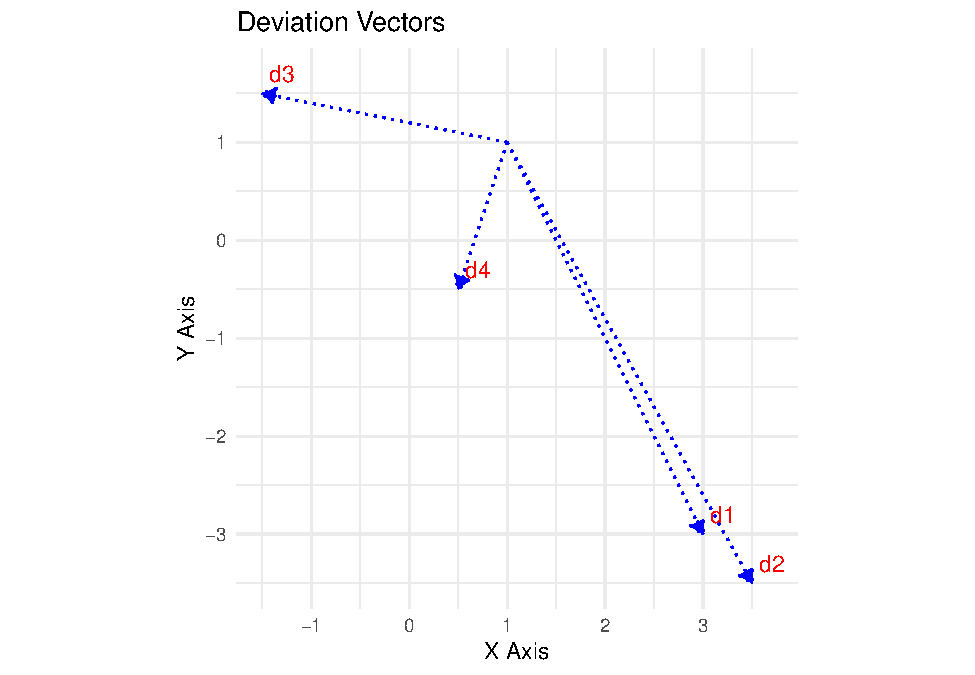
\includegraphics{CA1_files/figure-latex/unnamed-chunk-9-1.pdf}

\begin{Shaded}
\begin{Highlighting}[]
\CommentTok{\#Qtn 4}
\NormalTok{b }\OtherTok{\textless{}{-}} \FunctionTok{c}\NormalTok{(}\SpecialCharTok{{-}}\DecValTok{1}\NormalTok{,}\DecValTok{0}\NormalTok{,}\DecValTok{0}\NormalTok{,}\DecValTok{3}\NormalTok{)}
\NormalTok{means\_matrix }\OtherTok{\textless{}{-}} \FunctionTok{as.matrix}\NormalTok{(mean\_vectors[, }\DecValTok{2}\SpecialCharTok{:}\FunctionTok{ncol}\NormalTok{(mean\_vectors)])}
\NormalTok{y\_means }\OtherTok{\textless{}{-}}\NormalTok{ means\_matrix}\SpecialCharTok{\%*\%}\NormalTok{b}
\CommentTok{\#means for y1 to y5}
\NormalTok{y\_means}
\end{Highlighting}
\end{Shaded}

\begin{verbatim}
##          [,1]
## [1,] 20.23333
## [2,] 18.33333
## [3,] 17.23333
## [4,] 20.40000
## [5,] 17.93333
\end{verbatim}

\begin{Shaded}
\begin{Highlighting}[]
\CommentTok{\#now calculating the covariance matrix}
\NormalTok{data }\OtherTok{=}\NormalTok{ data }\SpecialCharTok{\%\textgreater{}\%} \FunctionTok{mutate}\NormalTok{(}\AttributeTok{Y =} \DecValTok{3}\SpecialCharTok{*}\NormalTok{NasHeight }\SpecialCharTok{{-}}\NormalTok{ MaxBreadth) }\CommentTok{\#the y value for each data data point}
\NormalTok{y\_data }\OtherTok{\textless{}{-}}\NormalTok{ data }\SpecialCharTok{\%\textgreater{}\%} \FunctionTok{select}\NormalTok{(TimePeriod, Y)}

\CommentTok{\#create an index to match data points ie 30 data points for 5 periods}
\NormalTok{index }\OtherTok{\textless{}{-}} \FunctionTok{rep}\NormalTok{(}\FunctionTok{seq}\NormalTok{(}\DecValTok{1}\NormalTok{,}\DecValTok{30}\NormalTok{), }\AttributeTok{times =} \DecValTok{5}\NormalTok{)}
\NormalTok{y\_data}\SpecialCharTok{$}\NormalTok{index }\OtherTok{\textless{}{-}}\NormalTok{ index}
\NormalTok{y\_data\_wide }\OtherTok{\textless{}{-}} \FunctionTok{pivot\_wider}\NormalTok{(y\_data, }\AttributeTok{names\_from =}\NormalTok{ TimePeriod, }\AttributeTok{values\_from =}\NormalTok{ Y) }\CommentTok{\#pivot data to use cov function}

\FunctionTok{head}\NormalTok{(y\_data\_wide)}
\end{Highlighting}
\end{Shaded}

\begin{verbatim}
## # A tibble: 6 x 6
##   index   `1`   `2`   `3`   `4`   `5`
##   <int> <dbl> <dbl> <dbl> <dbl> <dbl>
## 1     1    16    20    19    25    13
## 2     2    19    11    12    18    11
## 3     3    19    -3    12     6    43
## 4     4    13     5    20    18    26
## 5     5    26     9     1     5     3
## 6     6    30    21    10    19    30
\end{verbatim}

\begin{Shaded}
\begin{Highlighting}[]
\NormalTok{y\_data\_wide }\OtherTok{\textless{}{-}}\NormalTok{ y\_data\_wide }\SpecialCharTok{\%\textgreater{}\%} \FunctionTok{select}\NormalTok{(}\SpecialCharTok{{-}}\NormalTok{index) }\CommentTok{\#remove the index from cov calculation}
\NormalTok{y\_covariances }\OtherTok{\textless{}{-}} \FunctionTok{cov}\NormalTok{(y\_data\_wide)}
\NormalTok{y\_covariances}
\end{Highlighting}
\end{Shaded}

\begin{verbatim}
##            1         2         3          4           5
## 1 51.5643678  1.402299  23.32299  -7.924138   0.2229885
## 2  1.4022989 90.712644  -6.08046  29.862069   2.8850575
## 3 23.3229885 -6.080460 120.11609 -10.131034 -33.4321839
## 4 -7.9241379 29.862069 -10.13103  74.731034  14.6482759
## 5  0.2229885  2.885057 -33.43218  14.648276 165.0298851
\end{verbatim}

\end{document}
